\section{Array}

\begin{figure}[H]
        \centerline{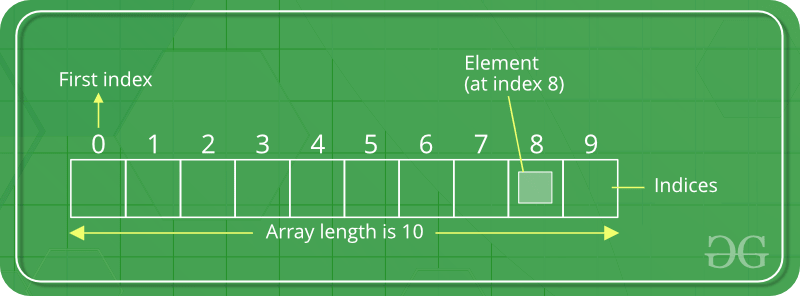
\includegraphics[scale=0.5]{figures/array/array-1}}
        \caption{Array: Geek for Geeks}
\end{figure}

Array adalah kumpulan item yang disimpan di lokasi memori yang berdekatan. Idenya adalah untuk menyimpan beberapa item dari jenis yang sama bersama-sama. Hal ini memudahkan untuk menghitung posisi setiap elemen hanya dengan menambahkan offset ke nilai dasar, yaitu, lokasi memori elemen pertama array (umumnya dilambangkan dengan nama array). Untuk kesederhanaan, kita dapat memikirkan sebuah array dengan tangga di mana pada setiap langkah ditempatkan sebuah nilai (katakanlah salah satu teman Anda). Di sini, Anda dapat mengidentifikasi lokasi teman Anda hanya dengan mengetahui jumlah langkah mereka. Array dapat berguna ketika kita harus memanipulasi hanya nilai tipe data tertentu. Seorang pengguna dapat memperlakukan daftar sebagai array. Namun, pengguna tidak dapat membatasi jenis elemen yang disimpan dalam daftar. Jika Anda membuat array menggunakan modul array, semua elemen array harus bertipe sama.

\section{Membuat Array}

Array di Python dapat dibuat dengan mengimpor modul array. array(data\_type, value\_list) digunakan untuk membuat array dengan tipe data dan daftar nilai yang ditentukan dalam argumennya.

\begin{lstlisting}[language=python, caption=Membuat Array]
# Python program to demonstrate
# Creation of Array
 
# importing "array" for array creations
import array as arr
 
# creating an array with integer type
a = arr.array('i', [1, 2, 3])
 
# printing original array
print ("The new created array is : ", end =" ")
for i in range (0, 3):
    print (a[i], end =" ")
print()
 
# creating an array with float type
b = arr.array('d', [2.5, 3.2, 3.3])
 
# printing original array
print ("The new created array is : ", end =" ")
for i in range (0, 3):
    print (b[i], end =" ")
\end{lstlisting}

Output:

\begin{lstlisting}
The new created array is :  1 2 3 
The new created array is :  2.5 3.2 3.3 
\end{lstlisting}

Beberapa tipe data disebutkan di bawah ini yang akan membantu dalam membuat array tipe data yang berbeda.

\begin{figure}[H]
        \centerline{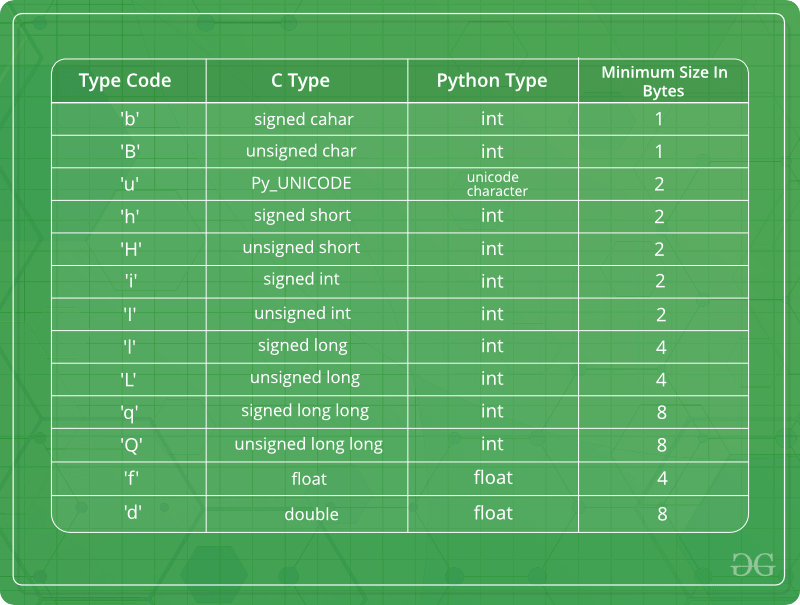
\includegraphics[scale=0.5]{figures/array/array-2}}
        \caption{Tipe Data Array: Geek for Geeks}
\end{figure}

\section{Menambah Elemen pada Array}
Elemen dapat ditambahkan ke Array dengan menggunakan fungsi insert() bawaan. Insert digunakan untuk menyisipkan satu atau lebih elemen data ke dalam array. Berdasarkan persyaratan, elemen baru dapat ditambahkan di awal, akhir, atau indeks array yang diberikan. append() juga digunakan untuk menambahkan nilai yang disebutkan dalam argumennya di akhir array.

\begin{lstlisting}[language=python, caption=Menambah Elemen Array]
# Python program to demonstrate
# Adding Elements to a Array

# importing "array" for array creations
import array as arr

# array with int type
a = arr.array('i', [1, 2, 3])


print ("Array before insertion : ", end =" ")
for i in range (0, 3):
	print (a[i], end =" ")
print()

# inserting array using
# insert() function
a.insert(1, 4)

print ("Array after insertion : ", end =" ")
for i in (a):
	print (i, end =" ")
print()

# array with float type
b = arr.array('d', [2.5, 3.2, 3.3])

print ("Array before insertion : ", end =" ")
for i in range (0, 3):
	print (b[i], end =" ")
print()

# adding an element using append()
b.append(4.4)

print ("Array after insertion : ", end =" ")
for i in (b):
	print (i, end =" ")
print()
\end{lstlisting}

Output:

\begin{lstlisting}
Array before insertion : 1 2 3 
Array after insertion :  1 4 2 3 
Array before insertion : 2.5 3.2 3.3 
Array after insertion :  2.5 3.2 3.3 4.4 
\end{lstlisting}

\section{Mengakses Elemen pada Array}

Untuk mengakses item array, gunakan nomor indeks. Gunakan operator indeks [ ] untuk mengakses item dalam array. Indeks harus berupa bilangan bulat.

\begin{lstlisting}[language=python, caption=Mengakses Elemen Array]
# Python program to demonstrate
# accessing of element from list

# importing array module
import array as arr

# array with int type
a = arr.array('i', [1, 2, 3, 4, 5, 6])

# accessing element of array
print("Access element is: ", a[0])

# accessing element of array
print("Access element is: ", a[3])

# array with float type
b = arr.array('d', [2.5, 3.2, 3.3])

# accessing element of array
print("Access element is: ", b[1])

# accessing element of array
print("Access element is: ", b[2])

\end{lstlisting}

Output:

\begin{lstlisting}
Access element is:  1
Access element is:  4
Access element is:  3.2
Access element is:  3.3
\end{lstlisting}

\section{Menghilangan Elemen pada Array}

Elemen dapat dihapus dari array dengan menggunakan fungsi remove() bawaan, tetapi akan muncul Error jika elemen tidak ada di set. Metode Remove() hanya menghapus satu elemen pada satu waktu, untuk menghapus rentang elemen, digunakan iterator. fungsi pop() juga dapat digunakan untuk menghapus dan mengembalikan elemen dari array, tetapi secara default hanya menghapus elemen terakhir dari array, untuk menghapus elemen dari posisi tertentu dari array, indeks elemen dilewatkan sebagai argumen ke metode pop().
Catatan – Hapus metode dalam Daftar hanya akan menghapus kemunculan pertama dari elemen yang dicari.

\begin{lstlisting}[language=python, caption=Menghilangkan Elemen Array]
# Python program to demonstrate
# Removal of elements in a Array

# importing "array" for array operations
import array

# initializing array with array values
# initializes array with signed integers
arr = array.array('i', [1, 2, 3, 1, 5])

# printing original array
print ("The new created array is : ", end ="")
for i in range (0, 5):
	print (arr[i], end =" ")

print ("\r")

# using pop() to remove element at 2nd position
print ("The popped element is : ", end ="")
print (arr.pop(2))

# printing array after popping
print ("The array after popping is : ", end ="")
for i in range (0, 4):
	print (arr[i], end =" ")

print("\r")

# using remove() to remove 1st occurrence of 1
arr.remove(1)

# printing array after removing
print ("The array after removing is : ", end ="")
for i in range (0, 3):
	print (arr[i], end =" ")
\end{lstlisting}

Output:

\begin{lstlisting}
The new created array is : 1 2 3 1 5 
The popped element is : 3
The array after popping is : 1 2 1 5 
The array after removing is : 2 1 5 
\end{lstlisting}

\section{Memotong pada Array}

Dalam array Python, ada beberapa cara untuk mencetak seluruh array dengan semua elemen, tetapi untuk mencetak rentang elemen tertentu dari array, kami menggunakan operasi Slice. Operasi irisan dilakukan pada array dengan menggunakan titik dua (:). Untuk mencetak elemen dari awal hingga rentang gunakan [:Index], untuk mencetak elemen dari penggunaan akhir [:-Index], untuk mencetak elemen dari Indeks tertentu hingga penggunaan akhir [Index:], untuk mencetak elemen dalam rentang, gunakan [ Start Index:End Index] dan untuk mencetak seluruh List dengan menggunakan operasi slicing, gunakan [:]. Selanjutnya, untuk mencetak seluruh array dalam urutan terbalik, gunakan [::-1].

\begin{lstlisting}[language=python, caption=Memotong Elemen Array]
# Python program to demonstrate
# slicing of elements in a Array

# importing array module
import array as arr

# creating a list
l = [1, 2, 3, 4, 5, 6, 7, 8, 9, 10]

a = arr.array('i', l)
print("Initial Array: ")
for i in (a):
	print(i, end =" ")

# Print elements of a range
# using Slice operation
Sliced_array = a[3:8]
print("\nSlicing elements in a range 3-8: ")
print(Sliced_array)

# Print elements from a
# pre-defined point to end
Sliced_array = a[5:]
print("\nElements sliced from 5th "
	"element till the end: ")
print(Sliced_array)

# Printing elements from
# beginning till end
Sliced_array = a[:]
print("\nPrinting all elements using slice operation: ")
print(Sliced_array)
\end{lstlisting}

Output:

\begin{lstlisting}
Initial Array: 
1 2 3 4 5 6 7 8 9 10 
Slicing elements in a range 3-8: 
array('i', [4, 5, 6, 7, 8])

Elements sliced from 5th element till the end: 
array('i', [6, 7, 8, 9, 10])

Printing all elements using slice operation: 
array('i', [1, 2, 3, 4, 5, 6, 7, 8, 9, 10])
\end{lstlisting}

\section{Mencari Elemen pada Array}

Untuk mencari elemen dalam array, kami menggunakan metode index() bawaan python. Fungsi ini mengembalikan indeks kemunculan pertama dari nilai yang disebutkan dalam argumen.

\begin{lstlisting}[language=python, caption=Mencari Elemen Array]
# Python code to demonstrate
# searching an element in array


# importing array module
import array

# initializing array with array values
# initializes array with signed integers
arr = array.array('i', [1, 2, 3, 1, 2, 5])

# printing original array
print ("The new created array is : ", end ="")
for i in range (0, 6):
	print (arr[i], end =" ")

print ("\r")

# using index() to print index of 1st occurrence of 2
print ("The index of 1st occurrence of 2 is : ", end ="")
print (arr.index(2))

# using index() to print index of 1st occurrence of 1
print ("The index of 1st occurrence of 1 is : ", end ="")
print (arr.index(1))
\end{lstlisting}

Output:

\begin{lstlisting}
The new created array is : 1 2 3 1 2 5 
The index of 1st occurrence of 2 is : 1
The index of 1st occurrence of 1 is : 0
\end{lstlisting}